\documentclass{beamer}
\usepackage{hyperref}
\usepackage{parskip}
\usepackage{verbatim}
\usepackage{tabularx}
\usepackage{amsmath}
\usepackage{comment}

% \usetheme{Madrid}
\usetheme{Boadilla}
% \usetheme{Montpellier}
\usepackage{Sweave}
\begin{document}
\Sconcordance{concordance:Lecture_3.2.tex:Lecture_3.2.Rnw:%
1 11 1 1 0 357 1}


\title{Intro to R Programming Day 3}
\author{Steve Pittard wsp@emory.edu}
\subtitle{Pittard Consulting}
\date{\today}

\maketitle


%% Data Frames continued
\section{ggplot2}


\begin{frame}[fragile]
\frametitle{ggplot2 - Intro}
R has a new graphics package called \textbf{ggplot2} that is based on a well developed
\textit{grammar of graphics}. The lattice package also attempts to adhere to a standard but
ggplot2 takes it to a new level. In general plots have:

\begin{itemize}

\item aesthetics
\begin{itemize}
\item coordinate positions (x,y)
\item element size, shape, and color
\end{itemize}

\item geometry 
\begin{itemize}
\item lines, points
\item segments, bars
\item text
\item element size, shape, and color
\end{itemize}

\end{itemize}
\end{frame}

\section{Terms}
\begin{frame}[fragile]
\frametitle{ggplot2 - Terms}
The terminology can be a little confusing:

\begin{itemize}
\item ggplot - The first version of the ggplot package
\item ggplot2 - an updated and the most recent version of the ggplot package
\item ggplot - is also an actual function in the ggplot2 package that allows you to build plots
\item qplot - a simplified function to ease your transition into the ggplot2 package
\item Many times I will just say or write ``ggplot'' as a synonym to ggplot2

\end{itemize}
\end{frame}


\begin{frame}[fragile]
\frametitle{ggplot2 - Terms}
\begin{itemize}
\item Like Latticce graphics ggplot can support grouping and distinction of data within a single of plot

\item ggplot can also support conditioning/panelling (though in ggplot it is called ``faceting'')

\item In practice and philosophy ggplot is closer to lattice graphics than it is to Base Graphics

\item This does not mean that the Base Graphics System is bad - just that it lacks a unifying philosophy. It is very powerful for creating graphics programmatically.

\item If you have the luxury of picking one then start with ggplot

\end{itemize}
\end{frame}




\section{Learning}
%  5 cool R visualizations 

\begin{frame}[fragile]
\frametitle{ggplot2 - Learning}
The idea is to first think of a plot in terms of these ideas after which you use specific ggplot2 commands to turn these ideas into an actual plot. 

ggplot2 provides two points of entry into the package.

\begin{itemize}
\item \textbf{qplot} - a simplified version of more involved ggplot commands. Sort of like training wheels for becoming accustomed to ggplot. It is meant to mimic the Base graphics \textbf{plot} command though \textbf{qplot} offers more generality.
\end{itemize}

qplot is the basic plotting function in the ggplot2 package. It is a convenient wrapper for creating a number of different types of plots using a consistent calling scheme.
\end{frame}


%  5 cool R visualizations 

\begin{frame}[fragile]
\frametitle{ggplot2 - Learning}
The idea is to first think of a plot in terms of these ideas after which you use specific ggplot2 commands to turn these ideas into an actual plot. 

ggplot2 provides two points of entry into the package.

\begin{itemize}

\item \textbf{ggplot} - which is the more complex yet far more flexible command for creating plots. I favor this approach since it allows one to assemble plots in layers. Most literature describing analysis and visualization using ggplot will use the more general approach.

\end{itemize}

The \textbf{ggplot} command can be used to declare the input data frame for a graphic and to specify the set of plot aesthetics intended to be common throughout all subsequent layers unless specifically overridden
\end{frame}

%  5 cool R visualizations 

\section{qplot}
\begin{frame}[fragile]
\frametitle{ggplot2 - qplot}
\scriptsize
\begin{verbatim}
qplot(mpg, wt, data=mtcars, main="MPG vs Wt",color=factor(cyl))
qplot(mpg, wt, data = mtcars, size = factor(cyl))
\end{verbatim}
\begin{center}
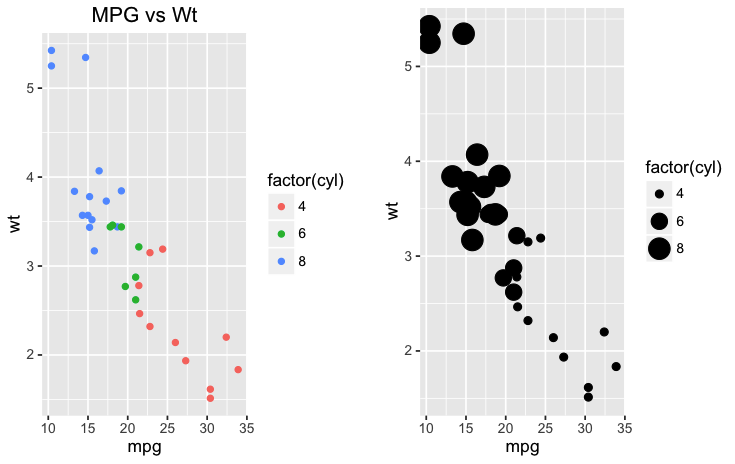
\includegraphics{../IMG/ggplot2_1.png}
\end{center}
\end{frame}

%

\begin{frame}[fragile]
\frametitle{ggplot2 - qplot}
You should explicitly make factors out of variables that you want to use as factors. Base and Lattice graphics are more forgiving about this than ggplot.
\scriptsize
\begin{verbatim}
qplot(mpg, wt, data=mtcars, main="MPG vs Wt",color=cyl)
\end{verbatim}
\begin{center}
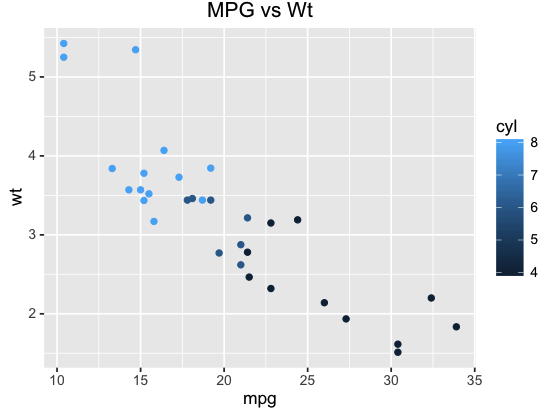
\includegraphics[height=7cm]{../IMG/qplot2_nofactor.png}
\end{center}
\end{frame}


%

\begin{frame}[fragile]
\frametitle{ggplot2 - qplot}
Here we make the cylinder variable into a factor
\scriptsize
\begin{verbatim}
mtcars$cyl <- factor(mtcars$cyl)
qplot(mpg, wt, data=mtcars, main="MPG vs Wt",color=cyl)
\end{verbatim}
\begin{center}
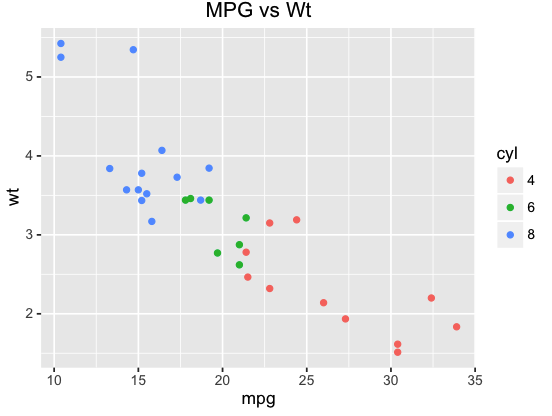
\includegraphics{../IMG/qplot_wfact.png}
\end{center}
\end{frame}


%  5 cool R visualizations 

\begin{frame}[fragile]
\frametitle{ggplot2 - qplot}
\scriptsize
\begin{verbatim}
mtcars$am <- factor(mtcars$am,labels=c("auto","manual"))
qplot(mpg, data=mtcars, geom="histogram",binwidth=5,fill=am) 
\end{verbatim}
\begin{center}
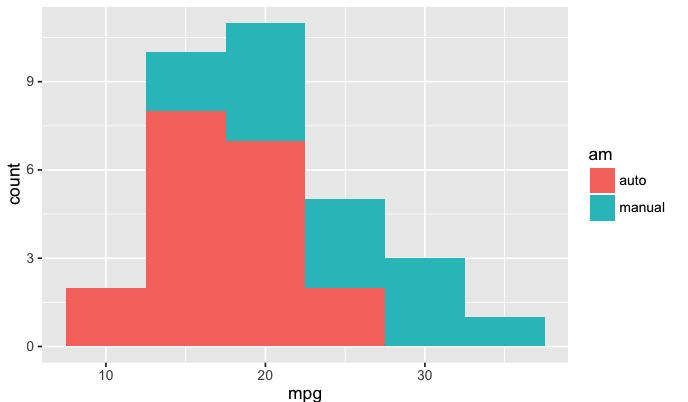
\includegraphics{../IMG/qplot3.png}
\end{center}
\end{frame}



% Barplot 

\begin{frame}[fragile]
\frametitle{ggplot2 - qplot}
\scriptsize
\begin{verbatim}
mtcars$cyl <- factor(mtcars$cyl)
qplot(factor(cyl),wt,data=mtcars,geom="boxplot",color=factor(cyl))
\end{verbatim}
\begin{center}
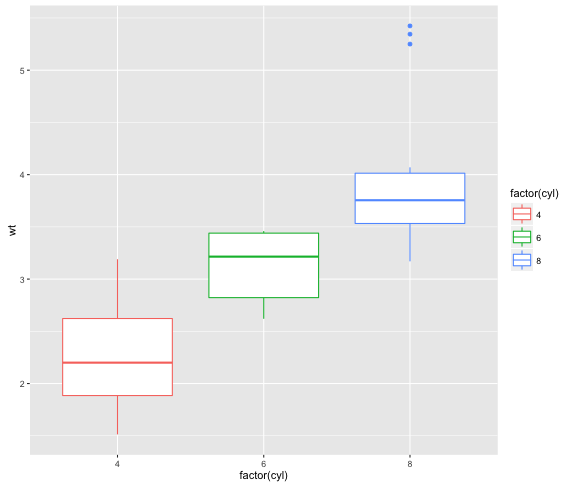
\includegraphics[height=7cm]{../IMG/ggplot_box.png}
\end{center}
\end{frame}


% Barplot 

\begin{frame}[fragile]
\frametitle{ggplot2 - qplot}So each geometry itself can have aesthetics.
\scriptsize
\begin{verbatim}
mtcars$cyl <- factor(mtcars$cyl)
qplot(mpg,wt, data=mtcars, geom="point", shape=cyl,size=1.2)
\end{verbatim}
\begin{center}
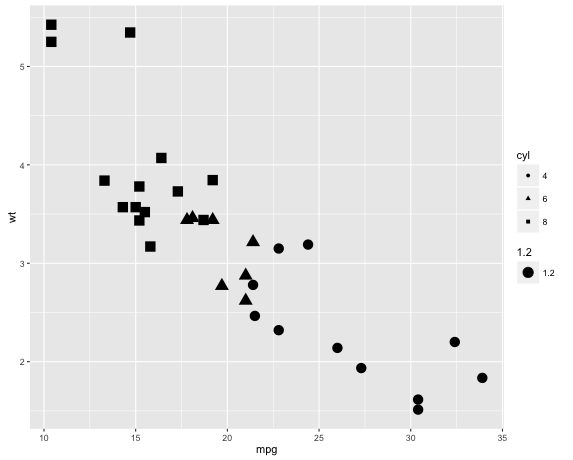
\includegraphics[height=7cm]{../IMG/qplot_geom_line.png}
\end{center}
\end{frame}


%

\begin{frame}[fragile]
\frametitle{ggplot2 - qplot}
\scriptsize
\begin{verbatim}
mtcars$cyl <- factor(mtcars$cyl)
qplot(mpg,wt, data=mtcars, geom="point", shape=cyl,size=1.2)
\end{verbatim}
\begin{center}
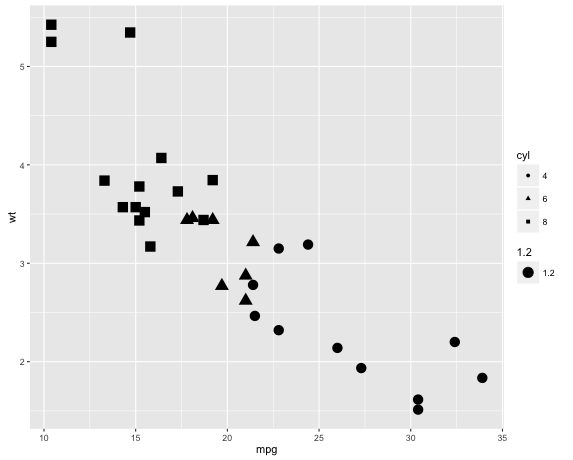
\includegraphics[height=7cm]{../IMG/qplot_geom_line.png}
\end{center}
\end{frame}


%
\begin{frame}[fragile]
\frametitle{ggplot2 - qplot}Each geometry can have aesthetics. Check out the \url{docs.ggplot2.org/} for information on what aesthetics are associated with a given geometry.

\scriptsize
\begin{center}
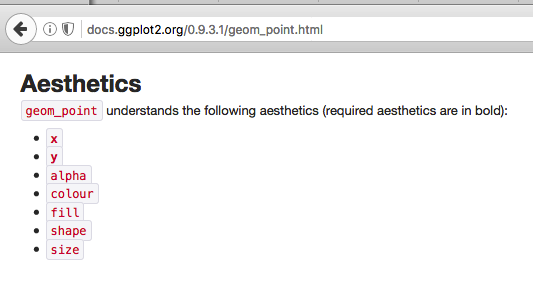
\includegraphics{../IMG/geom_ref.png}
\end{center}
\end{frame}


% Barplot 

\begin{frame}[fragile]
\frametitle{ggplot2 - qplot}
\scriptsize
\begin{verbatim}
qplot(mpg,wt, data=mtcars,geom="line",main="MPG vs Wt",color=cyl)
\end{verbatim}

\scriptsize
\begin{center}
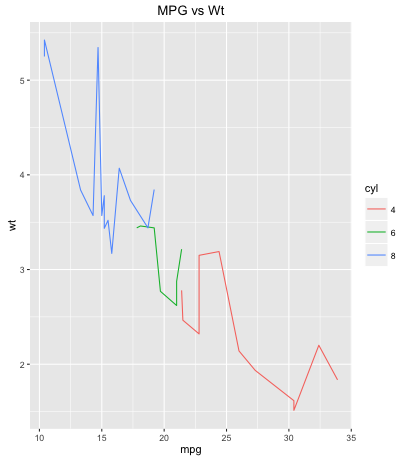
\includegraphics[height=7cm]{../IMG/qplot_line_color.png}
\end{center}
\end{frame}


% Barplot 

\begin{frame}[fragile]

The cool thing about the \textbf{bar} geom is that it will tabulate the number of observations in each category for you - unlike Base Graphics
\frametitle{ggplot2 - qplot}
\scriptsize
\begin{verbatim}
mtcars$cyl <- factor(mtcars$cyl)
qplot(cyl, data=mtcars, geom="bar",main="Cars by Cylinder")
\end{verbatim}

\scriptsize
\begin{center}
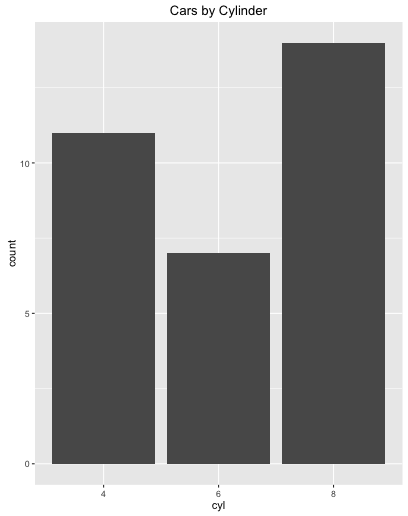
\includegraphics[height=6cm,width=6cm]{../IMG/bar_cnt.png}
\end{center}
\end{frame}


% Barplot 

\begin{frame}[fragile] 
\frametitle{ggplot2 - qplot}
\scriptsize
\begin{verbatim}
mtcars$am <- factor(mtcars$am)
qplot(cyl, data=mtcars, fill=am, geom="bar")
\end{verbatim}

\scriptsize
\begin{center}
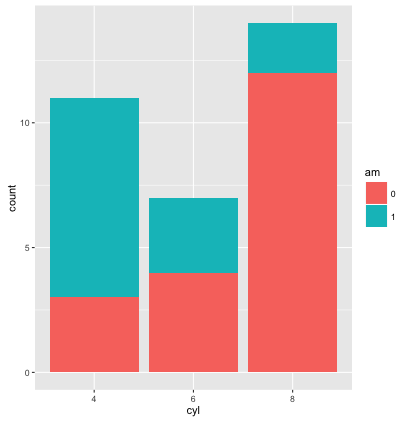
\includegraphics[height=7cm]{../IMG/qplot_am.png}
\end{center}
\end{frame}


% Barplot 

\begin{frame}[fragile]
\frametitle{ggplot2 - alpha}
\scriptsize
\begin{verbatim}
# Let's plot this with Base graphics
data(diamonds)  # A dataset on diamonds
plot(diamonds$carat,diamonds$price,main="Price of Diamonds")
grid()
\end{verbatim}
\begin{center}
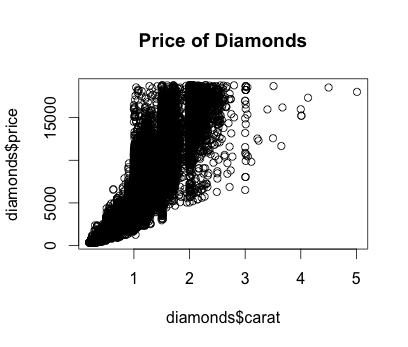
\includegraphics[height=8cm]{../IMG/qplot_base.png}
\end{center}
\end{frame}

%
\begin{frame}[fragile]
\frametitle{ggplot2 - alpha}
\scriptsize
\begin{verbatim}
# Let's plot this with lattice graphics
data(diamonds)  # A dataset on diamonds
xyplot(price~carat,data=diamonds,main="Price vs Caret",type=c("p","g"))
\end{verbatim}
\begin{center}
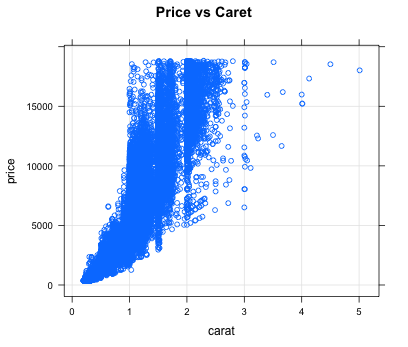
\includegraphics[height=7cm]{../IMG/lattice_diamonds.png}
\end{center}
\end{frame}
%

\begin{frame}[fragile]
\frametitle{ggplot2 - alpha}
\scriptsize
\begin{verbatim}
data(diamonds)  # A dataset on diamonds
title <- "Price vs Caret"
qplot(carat, price, data = diamonds, alpha = I(1/10),main=title)
\end{verbatim}
\begin{center}
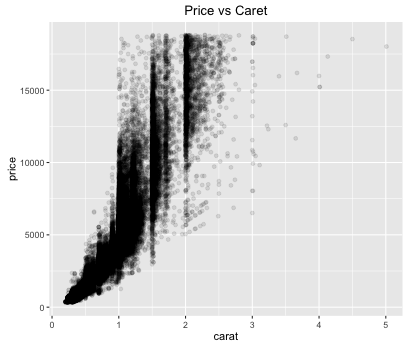
\includegraphics[height=7cm]{../IMG/qplot_alpha.png}
\end{center}
\end{frame}


%

\begin{frame}[fragile]
\frametitle{ggplot2 - alpha}
\scriptsize
\begin{verbatim}
data(diamonds)  # A dataset on diamonds
title <- "Price vs Caret"
qplot(carat, price, data = diamonds, alpha = I(1/100),main=title)
\end{verbatim}
\begin{center}
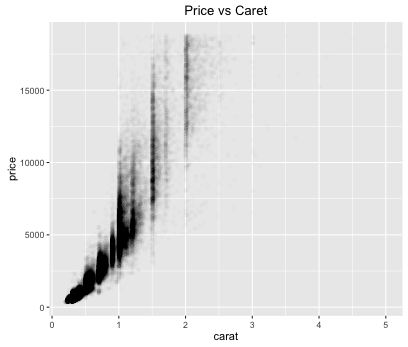
\includegraphics[height=7cm]{../IMG/qplot_dia2.png}
\end{center}
\end{frame}

%  5 cool R visualizations 

\begin{frame}[fragile]
\frametitle{ggplot2 - qplot}
\scriptsize
\begin{verbatim}
qplot(displ, hwy, data=mpg, facets = . ~ year) + geom_smooth()
\end{verbatim}
\begin{center}
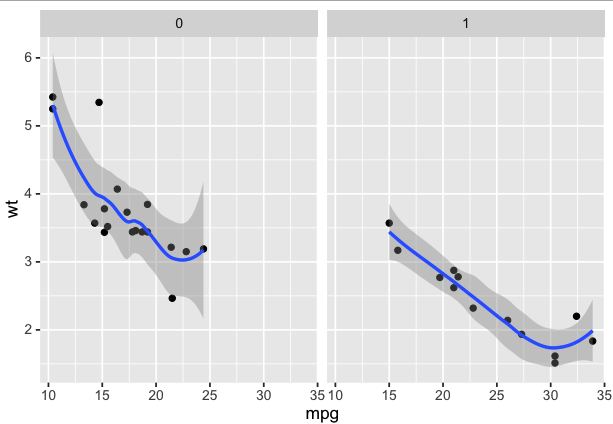
\includegraphics{../IMG/qplot2.png}
\end{center}
\end{frame}


%


%%% End of document
\end{document}
